% =============================================================================
% sections/design/rover/arm_vision_system.tex  -  Vision System
% Teams: arm
% Status: draft
%
% Images below are placeholders (teams/arm/figures/arm_camera_no_cv.png,
% teams/arm/figures/arm_camera_cv.png) - overwrite the same files with real
% arm-camera screenshots (raw frame / frame with detection overlay), no
% need to touch the LaTeX layout.
% =============================================================================

\todo[inline]{Write 1 short paragraph. Idea in plain words: we teach the
arm its positions by hand and save them (teach poses) — panel operations
just replay these saved positions. The camera is only needed because the
panel never stands exactly where it stood during teaching: it finds the
ArUco marker on the panel, computes how far the real panel is shifted
from the taught one, and shifts all saved positions by that amount. Also
tell the planner where the panel is, so the arm does not hit it.}

\autoref{fig:arm_camera_cv} shows the arm-camera view before and after
the detection overlay.

\begin{figure}[!htbp]
    \centering
    \begin{subfigure}[b]{0.48\textwidth}
        \centering
        
\includegraphics[width=\linewidth]{teams/arm/figures/panel_photo}
        \caption{Raw arm-camera frame}
    \end{subfigure}
    \hfill
    \begin{subfigure}[b]{0.48\textwidth}
        \centering
        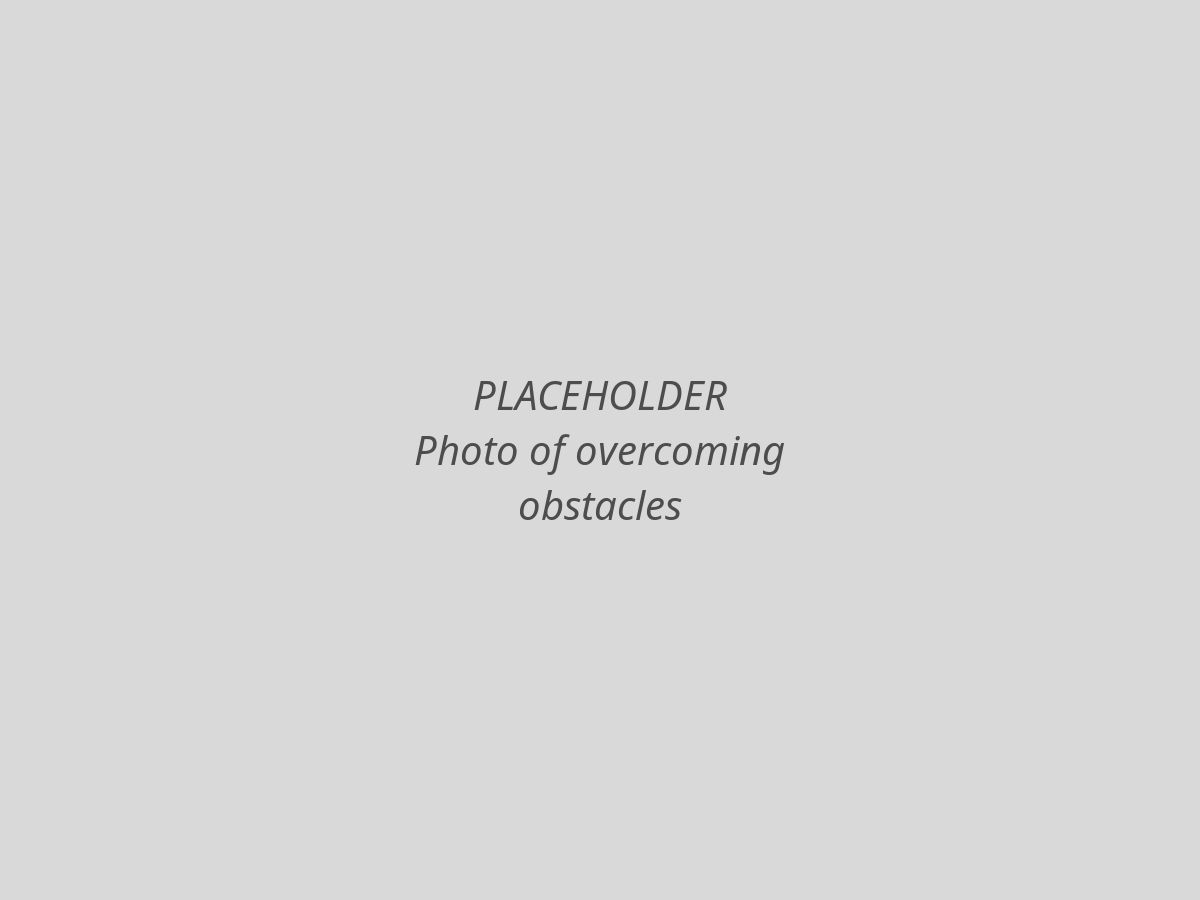
\includegraphics[width=\linewidth]{teams/arm/figures/panel_cv_photo}
        \caption{Frame with detection overlay}
    \end{subfigure}
    \caption{Arm-camera view without and with the vision pipeline}
    \label{fig:arm_camera_cv}
\end{figure}
